% Resume LaTeX creation test-1
\documentclass[a4paper,11pt]{article}

\usepackage[utf8]{inputenc}
\inputencoding{utf8}
\usepackage{textcomp}
\usepackage[scaled]{helvet}
\usepackage[a4paper,margin=0.75in, top=0.5in, bottom=0.4in]{geometry}

\thispagestyle{empty}
\usepackage{enumitem}
\usepackage{xcolor}
\usepackage[
  colorlinks=true,
  linkcolor=blue,
  urlbordercolor = {white}
]{hyperref}

\usepackage{multicol}
\usepackage{graphicx}
\usepackage[labelformat=empty]{caption}
\author{Svetlana Linuxenko}
\title{CV}
%\usepackage{tikz}
%
% ===== Document =====
%
\begin{document}

\begin{figure}
  \begin{minipage}{0.59\textwidth}
    {
\includegraphics[height=24pt]{s}}
%    \break
%    \Large{\sffamily{Front-End Developer}
  \end{minipage}
  \begin{minipage}{0.28\textwidth}
    \flushright
    \\\bigskip\break
%    {\sffamily{\large{Front-End Developer}}\hspace{22pt}\break
    \normalsize{
%    \href{https://twitter.com/linuxenko}{twitter/linuxenko}\hspace{24pt}\break
    {Contact e-mail address:}\hfill\break
    \href{mailto:svetlana@linuxenko.pro}{svetlana@linuxenko.pro}\hspace{24pt}\break
    \break
    \href{https://www.linuxenko.pro}{www.linuxenko.pro}\hspace{24pt}\break
    \href{https://github.com/linuxenko}{github.com/linuxenko}\hspace{24pt}\break
  }}
  \end{minipage}
  \begin{minipage}{0.12\textwidth}
    {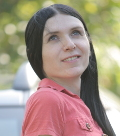
\includegraphics[height=66pt]{pic}}
  \end{minipage}
\end{figure}


% ===== Summary ======
%

\section*{Summary}
\paragraph{} I'm a software engineer with {\textbf {\small{10+}} years of experience working in research and commercial
conexts of both large and small companies. I build useful software by developing functional and correct
components, assembling them, releasing early. Experienced with modern front-end software design as well as
user interface and server side development.

%
% ===== Education =====
%

\section*{Education}
\begin{itemize}[itemsep=-4pt,label=]
  \item \textbf{Kyiv Polytechnic Institute}, NTUU ``KPI'' \\
  Software Engineer (Bachelor Degree) \hfill 2005-2010
\end{itemize}

%
% ===== Work Exp =====
%

\section*{Experience}
\begin{itemize}[itemsep=4pt,label=]

  \item \textbf{People.ai}, Kiev, Ukraine\\
    Senior Front-End Developer \hfill  2017

  \item \textbf{Dukascopy Bank SA}, Kiev, Ukraine\\
    Front-End Developer \hfill  2015 - 2016

  \item \textbf{Kaushan Media}, Kiev, Ukraine \\
    Front-End Developer \hfill  2014

\end{itemize}

%
% ===== Technical Skills =====
%

\section*{Technical}
\paragraph{} Familar with Banking, Game, eCommerce, Mobile, SmartTV applications development. Most comfortable development process for me is Test Driven in tandem with Scrum environment. Leading team, code review and refactoring. I prefer JavaScript, ES5,
sometimes ES6, client side and nodejs. Deep knowledge of Linux administration, shell scripting, vcs, mostly GIT, VIM addicted user.

\paragraph{} I work with: Ember.js, Angular.js, Backbone.js, React/Redux, Riot. Unit, Integration testing tools. Build tools, Continuous Integration systems. Experienced with general CSS frameworks, degradation strategies as well with material and mobile web design principles.
%
% ===== Authored =====
%
%\paragraph{} Big fan of computer science, i like investigate, sometimes invent algorithms and patterns from GOF to whole paradigms for my needs, storages and data formats, network protocols, etc.  Familar with Banking, Game, eCommerce, Mobile industry and more. Most comfortable development process for me is Test Driven in tandem with Scrum environment.
%Currently, I prefer following programming languages: JavaScript, ES5,
%sometimes ES6, C/C++, mostly SUS than POSIX, Java with some Spring Framework stuff. Deep knowledge of GNU/Linux administration, shell scripting, VCS, mostly GIT, vim addicted user.
%
%\paragraph{} As a front-end developer, i work with following things: ember.js, angular.js, backbone.js, react/redux, riot. Unit, Integration testing tools. Build tools, Continuous Integration system. Experienced with nodejs, isomorpic applications development, REST design, websockets. Work with general css frameworks, pre/postprocessors, css degradation strategies as well as material desing and mobile web design principles, animation and effects.
%
\section*{Authored}

\begin{itemize}[itemsep=4pt,label=]
  \item \textbf{Chkservice} \href{https://packages.debian.org/sid/chkservice}{packages.debian.org/sid/chkservice}\\
    GUI for systemd units configuration  \hfill  C/C++, s/DBUS, Ncurses

  \item \textbf{Unstuck-Webpack} \href{https://stuck.js.org}{stuck.js.org}\\
    GUI tool for webpack configuration \hfill  JavaScript, React, Material

  \item \textbf{CakeJS2 for SmartTV applications} \href{https://www.npmjs.com/package/cakejs2-spatial}{npmjs.com/package/cakejs2-spatial}\\
    React+Ember like framework \hfill  JavaScript, SmartTV \break
    with spatial navigation ready virtual-dom implementation\hfill\break
    Publication: \href{https://habrahabr.ru/post/320920/}{habrahabr/post/320920}

\end{itemize}
%
% ===== Technical Skills =====
%

%{\large \textbf{S}kills \& Qualifications} \hfill \href{https://github.com/linuxenko}{github.com/linuxenko}
%
%\begin{itemize}[itemsep=-2pt]
%  \item \textbf{ember}.js, \textbf{angular}.js, \textbf{backbone}.js, \textbf{react}/redux.js spa frameworks.
%    Test with \textbf{mocha}, \textbf{chai}, \textbf{sinon}, \textbf{jsdom}, \textbf{jest}, coverage reporting with \textbf{istanbull} and, of course,
%    \textbf{commonjs} helpers such as \textbf{browserify}, \textbf{webpack} and \textbf{babel}'s jsx transpiller, build tools.
%
%  \item Work with general \textbf{css frameworks, pre/postprocessors},  \textbf{css degradation} strategies as
%    well as \textbf{material} design and \textbf{mobile} web design principles.
%
%  \item Experienced with \textbf{nodejs isomorphic} applications development, \textbf{REST}ful http API design, \textbf{websockets},
%    basic \textbf{sql/nosql} database knowledge, \textbf{koa, express} nodejs frameworks.
%
%  \item Deep knowledge of GNU/\textbf{Linux} administration and \textbf{bash} scripting/writing tests. Continuous integration: \textbf{jenkins, travis}. Vcs, mostly \textbf{git}, \textbf{vim} addicted user.
%
%\end{itemize}
%



%
% ===== Open Source =====
%

%{\Large \textbf{O}pen Source}
%
%\begin{itemize}[label=]
%  
%  \item \textbf{Webpack Configurator Web Application} \hfill\href{https://stuck.js.org}{https://stuck.js.org}
%  \begin{itemize}[label=-]
%    \item Webpack quick project creation GUI tool that guide you throught all \\
%  the options. Created for those who don't like spend time for project configuration.
%  \end{itemize}
%
%  \item \textbf{Unix Console Markdown Pager} \hfill\href{https://lessmd.js.org}{https://lessmd.js.org}
%  \begin{itemize}[label=-]
%    \item Minimal marked based unix terminal document viewer/pager with many\\
%  features like markdown to terminal translation, file change watching and more.
%  \end{itemize}
%
%  \item \textbf{Conceptual Design of Mobile Things} \hfill\href{http://codepen.io/linuxenko}{http://codepen.io/linuxenko}
%  \begin{itemize}[label=-]
%    \item Implementation of the creative ideas on the ``paper''. Different mobile\\
%    related things such as design, behavior of different components.\\\medskip
%  \end{itemize}
%
%
%\end{itemize}

%
% ==== Preferred technologies ====
%

%{\Large \textbf{C}urrent Stack} 

%\begin{itemize}[label=]
%  \item \textbf{Programming}: es6, ember, webpack, babel, npm, react, redux, jest, node, express\\
%  \textbf{Tools}: vim, bash, docker, travis ci, jenkins, hreoku, phantomjs+casper, systemd, git\\
%  \textbf{OS}: Linux
%\end{itemize}

% {\Large \textbf{D}sdsfsfsdsdfgsdf}

% \begin{multicols}{6}
%   \begin{itemize}[label=-]
%     \setlength\itemsep{-5pt}
%     \item react
%     \item es6
%     \item npm
%     \item linux
%     \item node
%     \item ember
%     \item sass
%     \item less
%     \item css
%     \item redux
%     \item express
%     \item git
%     \item linux
%     \item webpack
%     \item docker
%     \item jest
%     \item jenkins
%     \item vim
%     \item mocha
%     \item systemd
%     \item rest
%     \item karma
%     \item rwd
%     \item[] \dots
%   \end{itemize}
% \end{multicols}

% \ \medskip

\vfill

\begin{center}
  \footnotesize{
  Check out my \href{https://github.com/linuxenko}{GitHub} profile,
  follow me on \href{https://twitter.com/linuxenko}{Twitter}.
  \\\medskip
  \textsf{\copyright} 2017 Svetlana Linuxenko
  }
\end{center}

\end{document}

